\documentclass[conference]{IEEEtran}
\IEEEoverridecommandlockouts
% The preceding line is only needed to identify funding in the first footnote. If that is unneeded, please comment it out.
\usepackage{cite}
\usepackage{amsmath,amssymb,amsfonts}
\usepackage{algorithmic}
\usepackage{graphicx}
\usepackage{textcomp}
\usepackage{xcolor}
\def\BibTeX{{\rm B\kern-.05em{\sc i\kern-.025em b}\kern-.08em
		T\kern-.1667em\lower.7ex\hbox{E}\kern-.125emX}}
\begin{document}
	
	\title{Report 5}
	
	\author{\IEEEauthorblockN{1\textsuperscript{st} Ali Ramezanzadeh}
		\IEEEauthorblockA{\textit{dept. of Electrical Engineering} \\
			\textit{Amirkabir University of Technology}\\
			Tehran, Iran\\
			ali.ramezan@aut.ac.ir}
		\and
		\IEEEauthorblockN{2\textsuperscript{nd} Arian Abdollahi}
		\IEEEauthorblockA{\textit{dept. of Electrical Engineering} \\
			\textit{Amirkabir University of Technology}\\
			Tehran, Iran\\
			arian.abdollahi@aut.ac.ir}
		\and
		\IEEEauthorblockN{3\textsuperscript{rd} Sina Shah Mohammadi}
		\IEEEauthorblockA{\textit{dept. of Electrical Engineering} \\
			\textit{Amirkabir University of Technology}\\
			Tehran, Iran\\
			alisinashahmohammadi@aut.ac.ir}}
	
	\maketitle

	
	\section{Introduction}
In this experiment, we want to design a lead and lag controller for an flexible joint robot.\newline
A flexible joint robot is a type of robot designed with joints that offer some degree of flexibility, compliance, or elasticity, distinguishing them from rigid robots. These robots incorporate elements like springs, elastic actuators, or specially designed mechanisms to allow controlled movement with some give or deformation at the joints. 

	\begin{figure}[htbp]
	\centerline{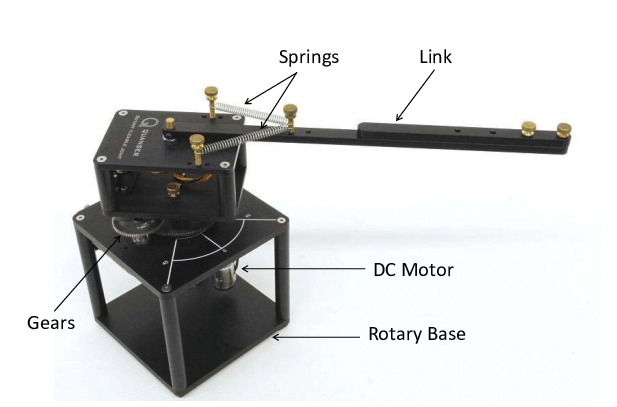
\includegraphics[width=0.7\linewidth]{1.jpg}}
	\caption{Flexible Joint Robot}
	\label{fig1}
\end{figure}

	\section{Mathematical Modeling}
We use the following diagram to derive the mathematical model of the system:

\begin{figure}[htbp]
	\centerline{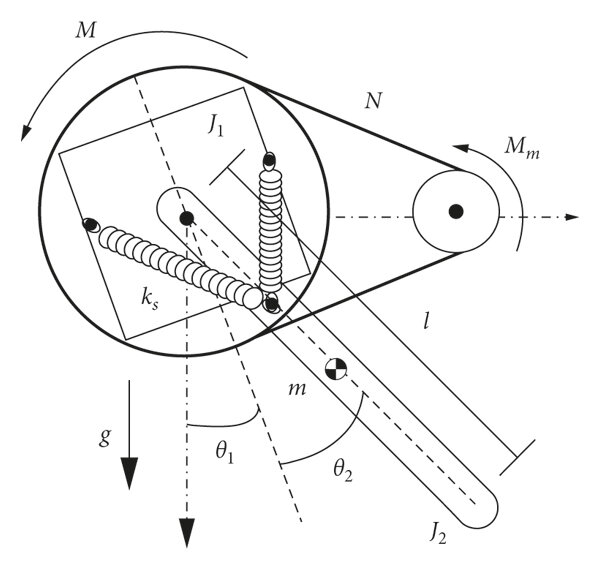
\includegraphics[width=0.7\linewidth]{2.jpg}}
	\caption{Flexible Joint Robot Model}
	\label{fig1}
\end{figure}

Using Lagrange-Hamilton, we arrive at the following equations.


\begin{equation}
	J_{eq} \ddot{\theta}+ J_{Arm}( \ddot{\theta}+\ddot{\alpha})=T_{output}-B_{eq}\dot{\theta}
\end{equation}


\begin{equation}
J_{Arm}( \ddot{\theta}+\ddot{\alpha})+K_{stiff}\alpha=0
\end{equation}

And we have the torque of a DC motor:

\begin{equation}
	T_{output}=\dfrac{\eta_{m}\eta_{g}K_{g}K_{m}(V_{m}-K_{g}K_{m}\dot{\theta})}{R_{m}}
\end{equation}
The selected state variables are:

\[
X=
\begin{pmatrix}
	\theta \\
	\dot{\theta}\\
	\alpha \\
	\dot{\alpha}\\
\end{pmatrix}
\]


Then, using the solve command in MATLAB, we solve the above equations and obtain the state-space matrices:

\[
A=
\begin{pmatrix}
	0 & 1 & 0 & 0 \\
	0 & {\frac{- (K_m  K_t  n_g  n_m   K_g^2 + B_{eq}  R_m)}{a}} & {\frac{K_{stiff}}{J_{eq}}} & 0 \\
	0 & 0 & 0 & 1 \\
	g &  {\frac{ (K_m  K_t  n_g  n_m   K_g^2 + B_{eq}  R_m)}{a}} & {\frac{-K_{stiff}(J_{arm}+J_{eq})}{J_{eq}J_{arm}}} & 0 \\
\end{pmatrix}
\]

\[
B=
\begin{pmatrix}
	0 \\
	\dfrac{K_{t}K_{g}\eta_{g}\eta_{m}}{J_{eq}R_{m}} \\
	0 \\
	-\dfrac{K_{t}K_{g}\eta_{g}\eta_{m}}{J_{eq}R_{m}} \\
\end{pmatrix}
\]

\[
C=
\begin{pmatrix}
	1 & 0&0 &0  \\
\end{pmatrix}
\qquad D=0
\]


 The Lead compensator is used to improve the transient response and has a positive phase, which increases the system's relative stability:
\[ G_c(s) = K \frac{s + Z}{s + P}, \quad |P| > |Z| \]


That we use this equation form for design:
\[
G_c(s) = K_c \alpha \frac{T s + 1}{\alpha T s + 1} = K_c \frac{s + \frac{1}{T}}{s + \frac{1}{\alpha T}}, \quad 0 < \alpha < 1
\]



The pole of the lead controller is always placed to the left of zero, and as the parameter ${\alpha}$ increases, this pole gets closer to zero. In the practical construction of this controller, there are certain constraints that typically require a minimum value for ${\alpha}$, which is generally 0.05. This suggests that the maximum phase that a lead controller can generate is approximately 65 degrees.\newline
${\phi_m}$represents the maximum phase that the controller can generate for a given value of ${\alpha}$, while ${\omega_m}$ indicates the frequency at which this maximum phase is achieved:

\begin{equation}
	\phi_m = PM_{desired}-PM+5
\end{equation}

\begin{equation}
	\sin(\phi_m) = \frac{1 - \alpha}{1 + \alpha}
\end{equation}
\begin{equation}
	\omega_m = \frac{1}{\sqrt{\alpha}T} 
\end{equation}
Thus:
\[ \phi_m = 12.5  \qquad  \alpha = .6456 \]\\\[ \omega_m = 10.5 \qquad T =0.1185 \]

\begin{equation}
	\alpha = \frac{Z}{P} \quad \omega_m = \sqrt{ZP}
\end{equation}
Thus:
\[ Z = 8.367 \quad P = 13.07\]

this is the bode diagram of the system before applying the lead controller:

\begin{figure}[htbp]
	\centerline{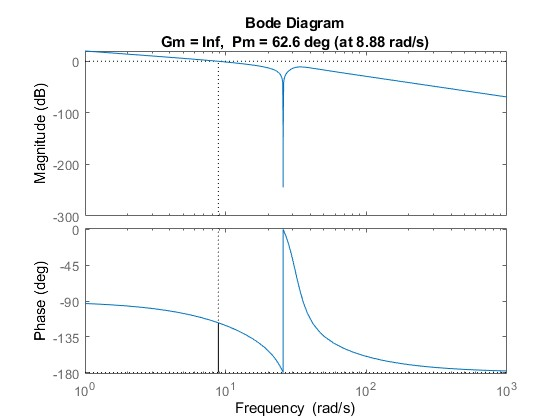
\includegraphics[width=0.9\linewidth]{3.jpg}}
	\caption{System Bode Diagram}
	\label{fig3}
\end{figure}
\newpage
And this is the bode diagram of the system after applying the lead controller:

\begin{figure}[htbp]
	\centerline{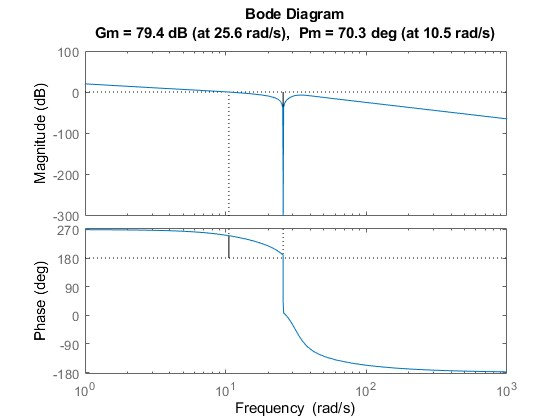
\includegraphics[width=0.9\linewidth]{4.jpg}}
	\caption{System Bode Diagram With Lead Controller}
	\label{fig4}
\end{figure}

	\section{Simulink}
	
	After all we plant the system on simulink. Here is the result:

\begin{figure}[htbp]
	\centerline{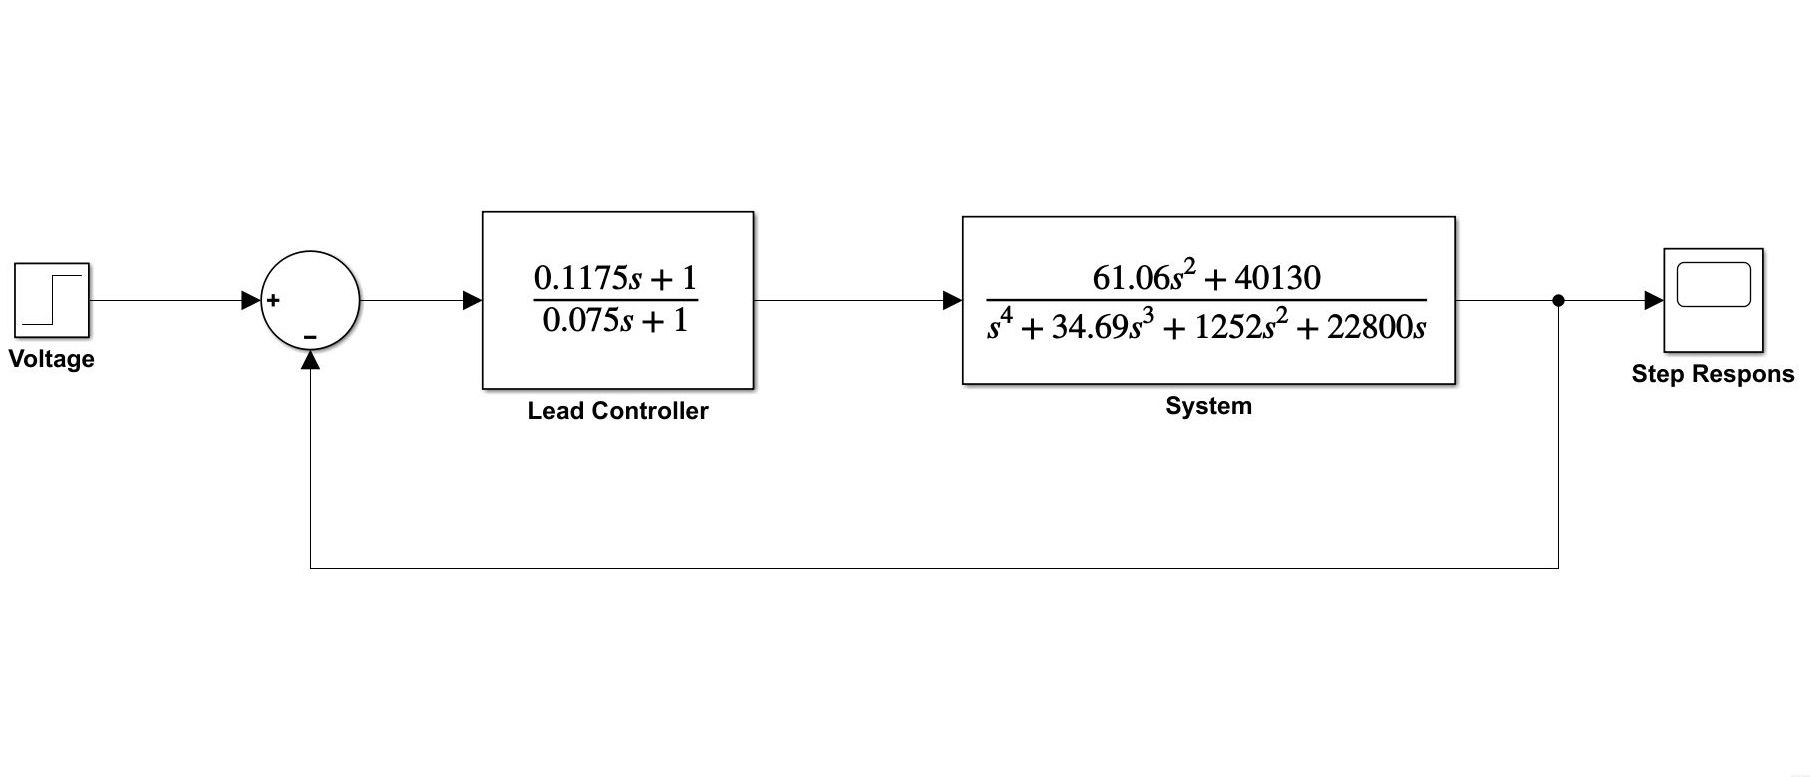
\includegraphics[width=0.9\linewidth]{5.jpg}}
	\caption{System With Lead Controller Simulink}
	\label{fig4}
\end{figure}

\end{document}

